\documentclass[12pt, a4paper]{article}

\usepackage{array}
\usepackage[portuguese]{babel}
\usepackage{float}
\usepackage[a4paper, margin=2cm]{geometry}
\usepackage{graphicx}
\usepackage{hyperref}
\usepackage{pdfpages}
\usepackage{setspace}

\title{\textbf{Interface Pessoa-Máquina \\ \large Trabalho Prático -- Fase II}}
\date{4 de maio de 2025}
\author{Grupo 12 \\
    \url{https://github.com/UMinho-ENGINF-IPM/trabalho-pr-tico-gp25_12}}

\begin{document}

\begin{center}
    
\includegraphics[width=0.25\textwidth]{res/cover/school-of-engineering.eps}
\end{center}

{\let\newpage\relax\maketitle}
\maketitle
\thispagestyle{empty}

\chardef\_=`_
\onehalfspacing
\setlength{\parskip}{\baselineskip}
\setlength{\intextsep}{2\baselineskip}
\setlength\belowcaptionskip{-\baselineskip}
\setlength{\parindent}{0pt}
\def\arraystretch{1.5}

\vspace{2cm}
\begin{center}
    \begin{tabular}{>{\centering}p{0.25\textwidth}
                    >{\centering}p{0.25\textwidth}
                    >{\centering\arraybackslash}p{0.25\textwidth}}
        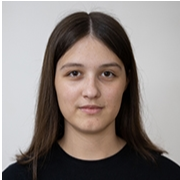
\includegraphics[width=3.5cm]{res/cover/A104437.png} &
        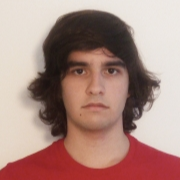
\includegraphics[width=3.5cm]{res/cover/A104348.png} &
        
\includegraphics[width=3.5cm]{res/cover/A104263.png}  \\

        Ana Oliveira & Humberto Gomes & Inês Marques \\
        A104437      & A104348        & A104263
    \end{tabular}

    \begin{tabular}{>{\centering}p{0.25\textwidth}
                    >{\centering\arraybackslash}p{0.25\textwidth}}
        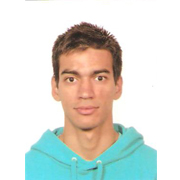
\includegraphics[width=3.5cm]{res/cover/A76350.jpg} &
        
\includegraphics[width=3.5cm]{res/cover/A104179.png} \\

        Rafael Vilas Boas & Sara Lopes \\
        A76350            & A104179
    \end{tabular}
\end{center}

\begin{abstract}
    \noindent
\end{abstract}

\section{Alterações ao Modelo da Interface}

\section{Componentes Implementados}

\section{Páginas Implementadas}

\section{Tecnologias Utilizadas}

\section{Conclusão e Trabalho Futuro}

\begingroup
\section{Bibliografia}
\renewcommand{\section}[2]{}

\begin{thebibliography}{9}
    \bibitem{figma}
        ``Figma: Collaborative Interface Design Tool.''. Figma. Accessed: Mar. 13, 2025. [Online.]
        Available: \url{https://www.figma.com/}
\end{thebibliography}
\endgroup

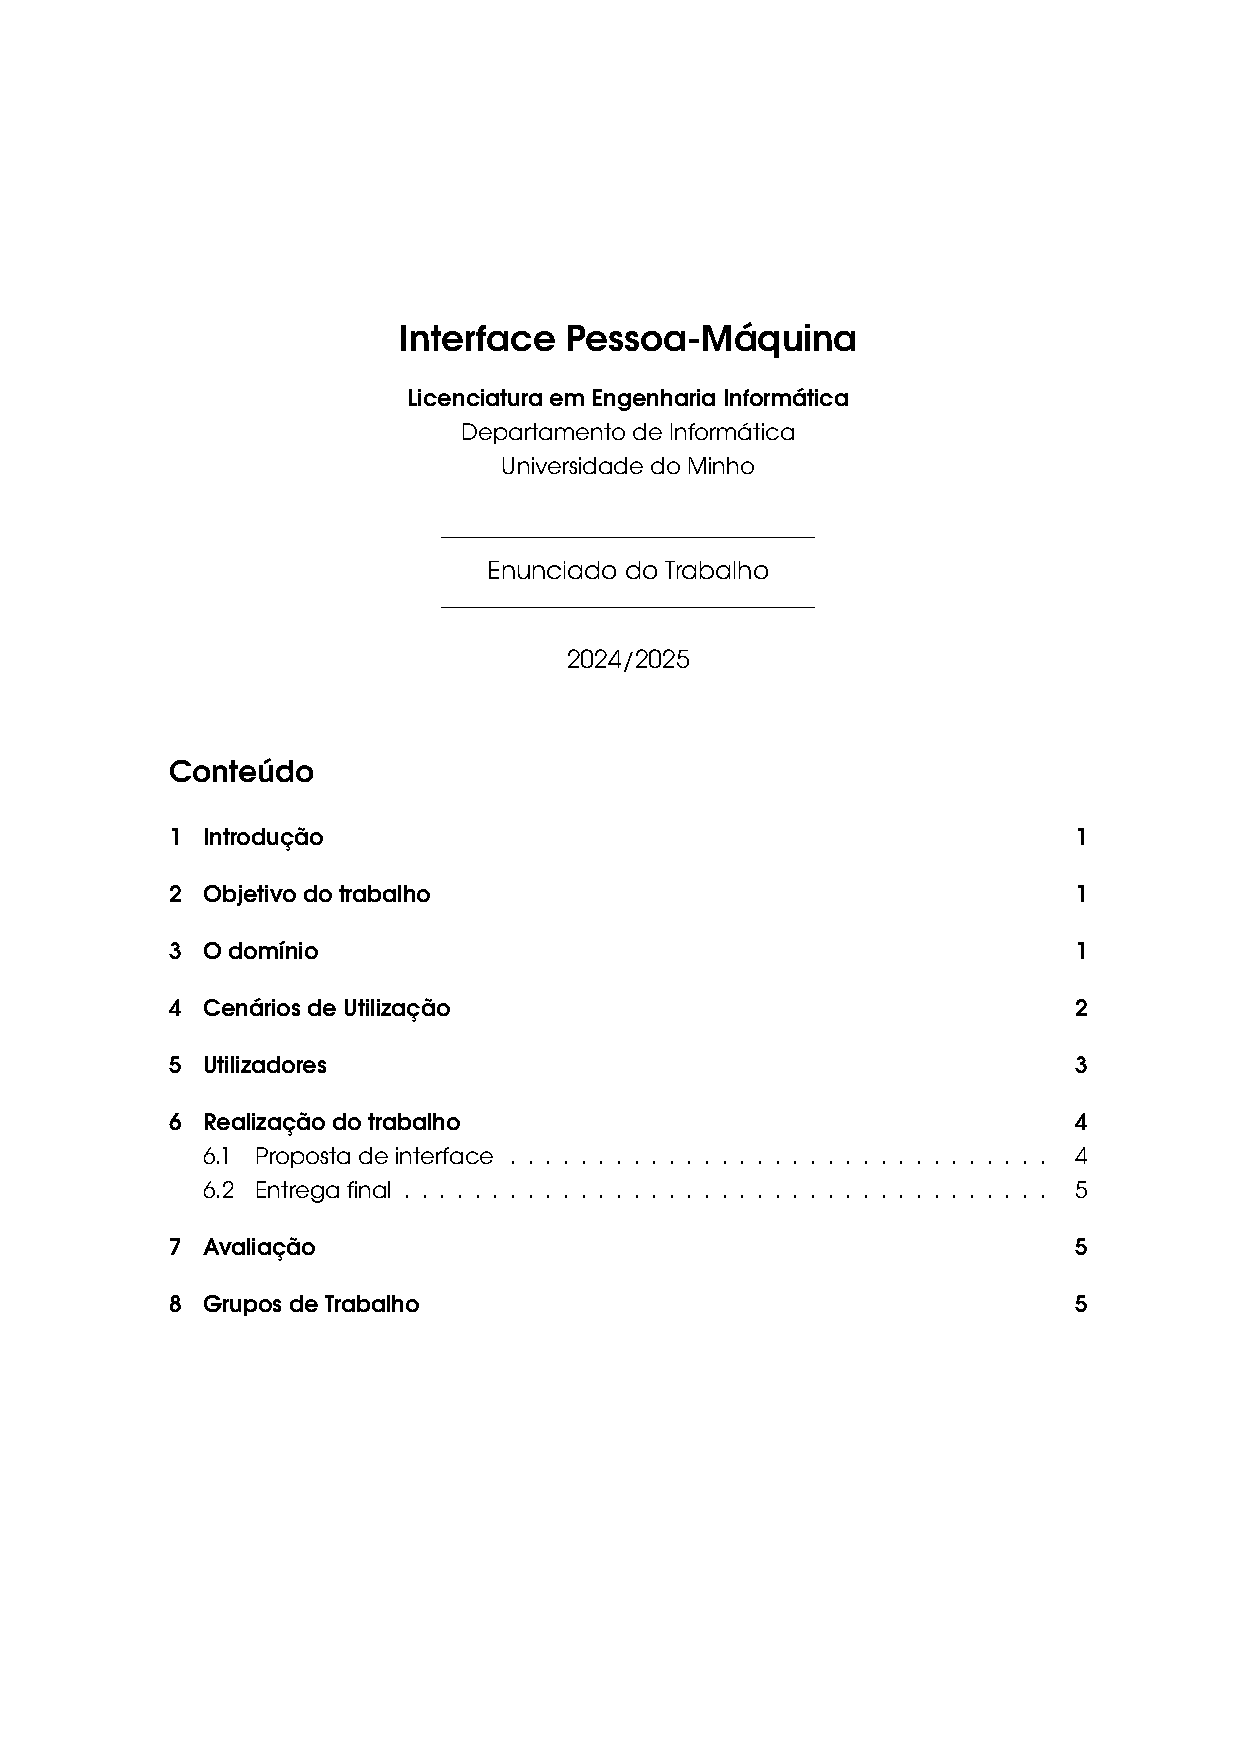
\includepdf[pages=1,pagecommand=\section{Anexo -- Enunciado do Trabalho}\thispagestyle{empty}]
    {../Assignment.pdf}
\includepdf[pages=2-]{../Assignment.pdf}

\end{document}
